\documentclass{article}
\usepackage[preprint]{neurips_2025}
\usepackage[utf8]{inputenc}
\usepackage[T1]{fontenc}
\usepackage{amsmath,amssymb,booktabs,graphicx,microtype,url}
\setlength{\textfloatsep}{6pt plus 2pt minus 1pt}
\setlength{\floatsep}{5pt plus 2pt minus 1pt}
\setlength{\intextsep}{6pt plus 2pt minus 1pt}
\title{Generating Chest X-rays with a Hierarchical Variational Autoencoder}
\author{Xinying (Ashley) Liu\\University of California, San Diego}
\begin{document}
\maketitle
\begin{abstract}
We implement a hierarchical variational autoencoder (VAE) in PyTorch and train it on pediatric chest radiographs. A 128-dimensional global latent represents coarse anatomy; a conditional 32$\times$32 spatial latent provides local variation. Structure-aware reconstruction losses improve validation SSIM from 0.690 to 0.754. Independent prior sampling yields recognizable but smooth chest X-rays; optional decoder-only adversarial refinement reduces matched-validation FID from 216.52 to 210.14. We distinguish reconstruction quality from generative fidelity throughout.
\end{abstract}

\section{Approach}
\textbf{Dataset.} We use the Kaggle Chest X-Ray Images (Pneumonia) dataset specified in the assignment. Its original training directory contains 5,216 images, split once by class (seed 2026) into 4,694 training and 522 validation images. Each image is converted to grayscale and resized to $128\times128$; the provided test directory is held out and not included in the results below.

\textbf{Model.} We implement an encoder, Gaussian reparameterization, conditional prior, and convolutional-residual decoder. The hierarchical posterior factorizes as $q_\phi(z_g\mid x)q_\phi(z_\ell\mid x,z_g)$, with global latent $z_g\in\mathbb R^{128}$ and spatial latent $z_\ell\in\mathbb R^{8\times32\times32}$. For \emph{new} images, we sample $z_g\sim\mathcal N(0,I)$ and $z_\ell\sim p_\theta(z_\ell\mid z_g)$, then decode without using an input chest X-ray. No deterministic encoder--decoder skip connections are present. Our main H3B objective is
\begin{equation}
\mathcal L=\mathrm{MSE}_{\rm sum}+48(1-\mathrm{SSIM})+32\mathcal L_{\rm edge}
+\beta_t\bigl(\mathrm{KL}_g+0.35\,\mathrm{KL}_\ell\bigr),
\end{equation}
with a ten-epoch KL warm-up to $\beta_t=1$. This is a hybrid reconstruction-regularized VAE objective, not an exact negative ELBO \citep{kingma2014auto}. H1 uses pixel MSE only; H2 adds SSIM and Sobel edge terms with a 16$\times$16 local latent; H3B enlarges that grid to 32$\times$32 and downweights local KL. Training uses AdamW (initial learning rate $1.5\times10^{-4}$, weight decay $10^{-4}$), batch size 16, 50 epochs, gradient clipping, and EMA ($0.999$). We select the checkpoint using validation loss.

\section{Experimental results}
\textbf{Reconstruction.} The held-out validation MSE/SSIM is 0.00362/0.690 for H1, 0.00352/0.697 for H2, and \textbf{0.00247/0.754} for H3B. This progression indicates better input-conditioned reconstruction under the combined architecture/loss changes, but does not in itself establish improved prior generation. In the saved H3B history, both train and validation objectives decrease across 50 epochs (Figure~\ref{fig:visual}).

\textbf{Generation.} We report ImageNet Inception-based Fr\'echet Inception Distance (FID) \citep{heusel2017gans} and Inception Score (IS) \citep{salimans2016improved} for 522 independent prior samples against the 522-image validation set. As an \emph{optional extension}, H6A freezes the H3B encoder and both priors, fine-tuning only the decoder for 15 epochs with a weak spectral-normalized patch-discriminator objective on reconstructions and prior samples. H6A is not presented as a pure-VAE training run.
\begin{table}[!ht]
\centering
\caption{Matched validation generation (seed 2026, $n_{\rm real}=n_{\rm fake}=522$); FID/KID lower, IS higher.}
\vspace{-4pt}
\small
\begin{tabular}{@{}lrrr@{}}
\toprule
Model & FID$\downarrow$ & KID$\downarrow$ & IS$\uparrow$ \\
\midrule
H3B, hierarchical VAE & 216.52 & 0.2725 & 2.287 \\
H6A, decoder refinement & \textbf{210.14} & \textbf{0.2612} & \textbf{2.321} \\
\bottomrule
\end{tabular}
\vspace{-7pt}
\end{table}

\begin{figure}[!ht]
\centering
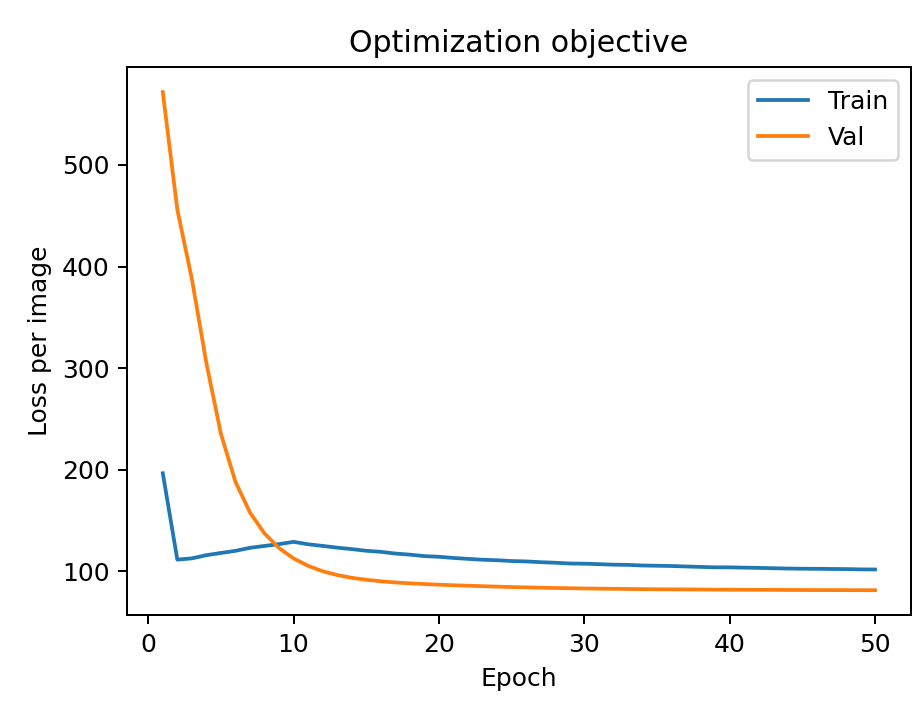
\includegraphics[width=.61\textwidth]{figs/report_training_objective.png}
\par\vspace{2pt}
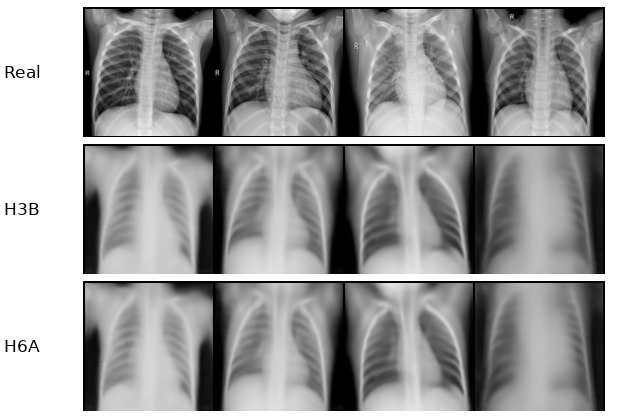
\includegraphics[width=.61\textwidth]{figs/report_generation_examples.png}
\caption{\textbf{Top:} H3B train/validation objective across 50 epochs. \textbf{Bottom:} top row shows \emph{unpaired} real validation images; next rows show H3B/H6A unconditional samples from matched latent draws. The synthetic images are not reconstructions of the real examples.}
\label{fig:visual}
\vspace{-5pt}
\end{figure}

\textbf{Interpretation and limitations.} Samples generally recover the lung-field silhouette and mediastinum, but ribs and fine pulmonary markings are too smooth. The modest FID reduction does not establish statistical significance with only 522 validation images. A separate detail-latent ablation produced sharper reconstructions but much worse prior samples, reinforcing that reconstruction scores cannot substitute for generative evaluation. ImageNet-based FID/IS are imperfect for radiographs, and these synthetic images are not intended for clinical use.

\section{Conclusion}
A from-scratch hierarchical VAE can generate recognizable chest radiographs, and structural losses improve reconstruction. Limited adversarial decoder refinement helps image-distribution metrics slightly, but high-frequency realism remains an unresolved limitation.

\vspace{-3pt}
\begin{thebibliography}{9}
\small
\bibitem[Kingma and Welling(2014)]{kingma2014auto} D. Kingma and M. Welling. Auto-Encoding Variational Bayes. \emph{ICLR}, 2014.
\bibitem[Heusel et~al.(2017)]{heusel2017gans} M. Heusel et al. GANs trained by a two time-scale update rule converge to a local Nash equilibrium. \emph{NeurIPS}, 2017.
\bibitem[Salimans et~al.(2016)]{salimans2016improved} T. Salimans et al. Improved techniques for training GANs. \emph{NeurIPS}, 2016.
\end{thebibliography}
\end{document}
